%% ----------------------------------------------------------------
%% Chapter 3 -- System Design & Architecture
%% ----------------------------------------------------------------
\chapter{System Design \& Architecture}
\label{chap:sysdesign}

This segment describes how an integrated Sensing \& Communication (ISAC) platform will be designed for continuous object tracking indoors where GPS is unavailable. The described system uses microcontrollers on the ``edge'' instead of expensive Software Defined Radio (SDR) platforms. Using both millimeter wave (mmWave) sensing and communication below 6~GHz frequencies, this system can address the randomness associated with signal propagation in indoor environments.

\section{Problem Statement}
\label{sec:problem}

ISACs using one modality fail in indoor areas that have obstructions since both modalities have inverse strengths and complementary failure modes. For example, a 24~GHz frequency modulation carrier wave (FMCW) radar has a very high spatial resolution ($\pm$0.15~m) in a $\pm$60° FOV at 10 to 24~Hz, capturing detailed micro-Doppler signatures of human motion. Unfortunately, FMCW radars are identity blind. Additionally, mmWave signals tend to experience minimal diffraction when interacting with solid obstacles; therefore, complete target loss occurs during occlusion events, and often produces ``ghost'' targets resulting from multipath reflections.

IEEE 802.11mc Fine Time Measurements at 2.4~GHz is inherently identity aware and associates requests with specific MAC addresses. As such, the 2.4~GHz carrier diffracts around typical building materials allowing tracking to continue even under extreme conditions. However, FTM updates are bursty. Due to receiver saturation and near-field multipath, radial error increases between 1.5 to 4.8~m at close proximity~\cite{aggarwal_wifi}.

The fusion of those two sensor systems presents two major technological challenges. The first one is the Synchronization Gap and Freshness Blindness. Standard Kalman Filters have to be updated synchronously. In other words, if you are trying to fuse high-speed radar with bursty Wi-Fi at 1~Hz per update, there will be many time periods where your standard Kalman Filter can't tell whether it should continue using stale Wi-Fi or fresh radar because both are given equal weightage during those inter-update intervals. As a result of this behavior, you get a ``staircase'' effect - your track will stall after each update until the next Wi-Fi registration. Thus, the architecture needs a real-time mechanism that is able to monitor the age of information and dynamically adjust the covariance of all aging measurement values based on their ages.

The second hurdle is geometric mismatch. The output of the sensors has different spatial geometries. Radar determines target positions in 2D Cartesian space $(x,y)$, while FTM determines only a single one dimensional scalar distance without determining angle. Therefore, converting the scalar distance from the radar into Cartesian space requires knowing an angular heading, which is exactly where radar fails due to occlusion. Therefore, there is a mandatory need for transforming into polar coordinates, isolating the radial component as an independent Wi-Fi backup solution during times when the radar loses its angular vector.

\section{Hardware Architecture}
\label{sec:hardware}

The sensing node uses the dual core ESP32-S3 microprocessor as FTM initiator, radar parser and also as edge inference processor. When the hardware boots up, the firmware runs permanent Wi-Fi calibration routines so that the radio operates stably.

\begin{figure}[htbp]
\centering
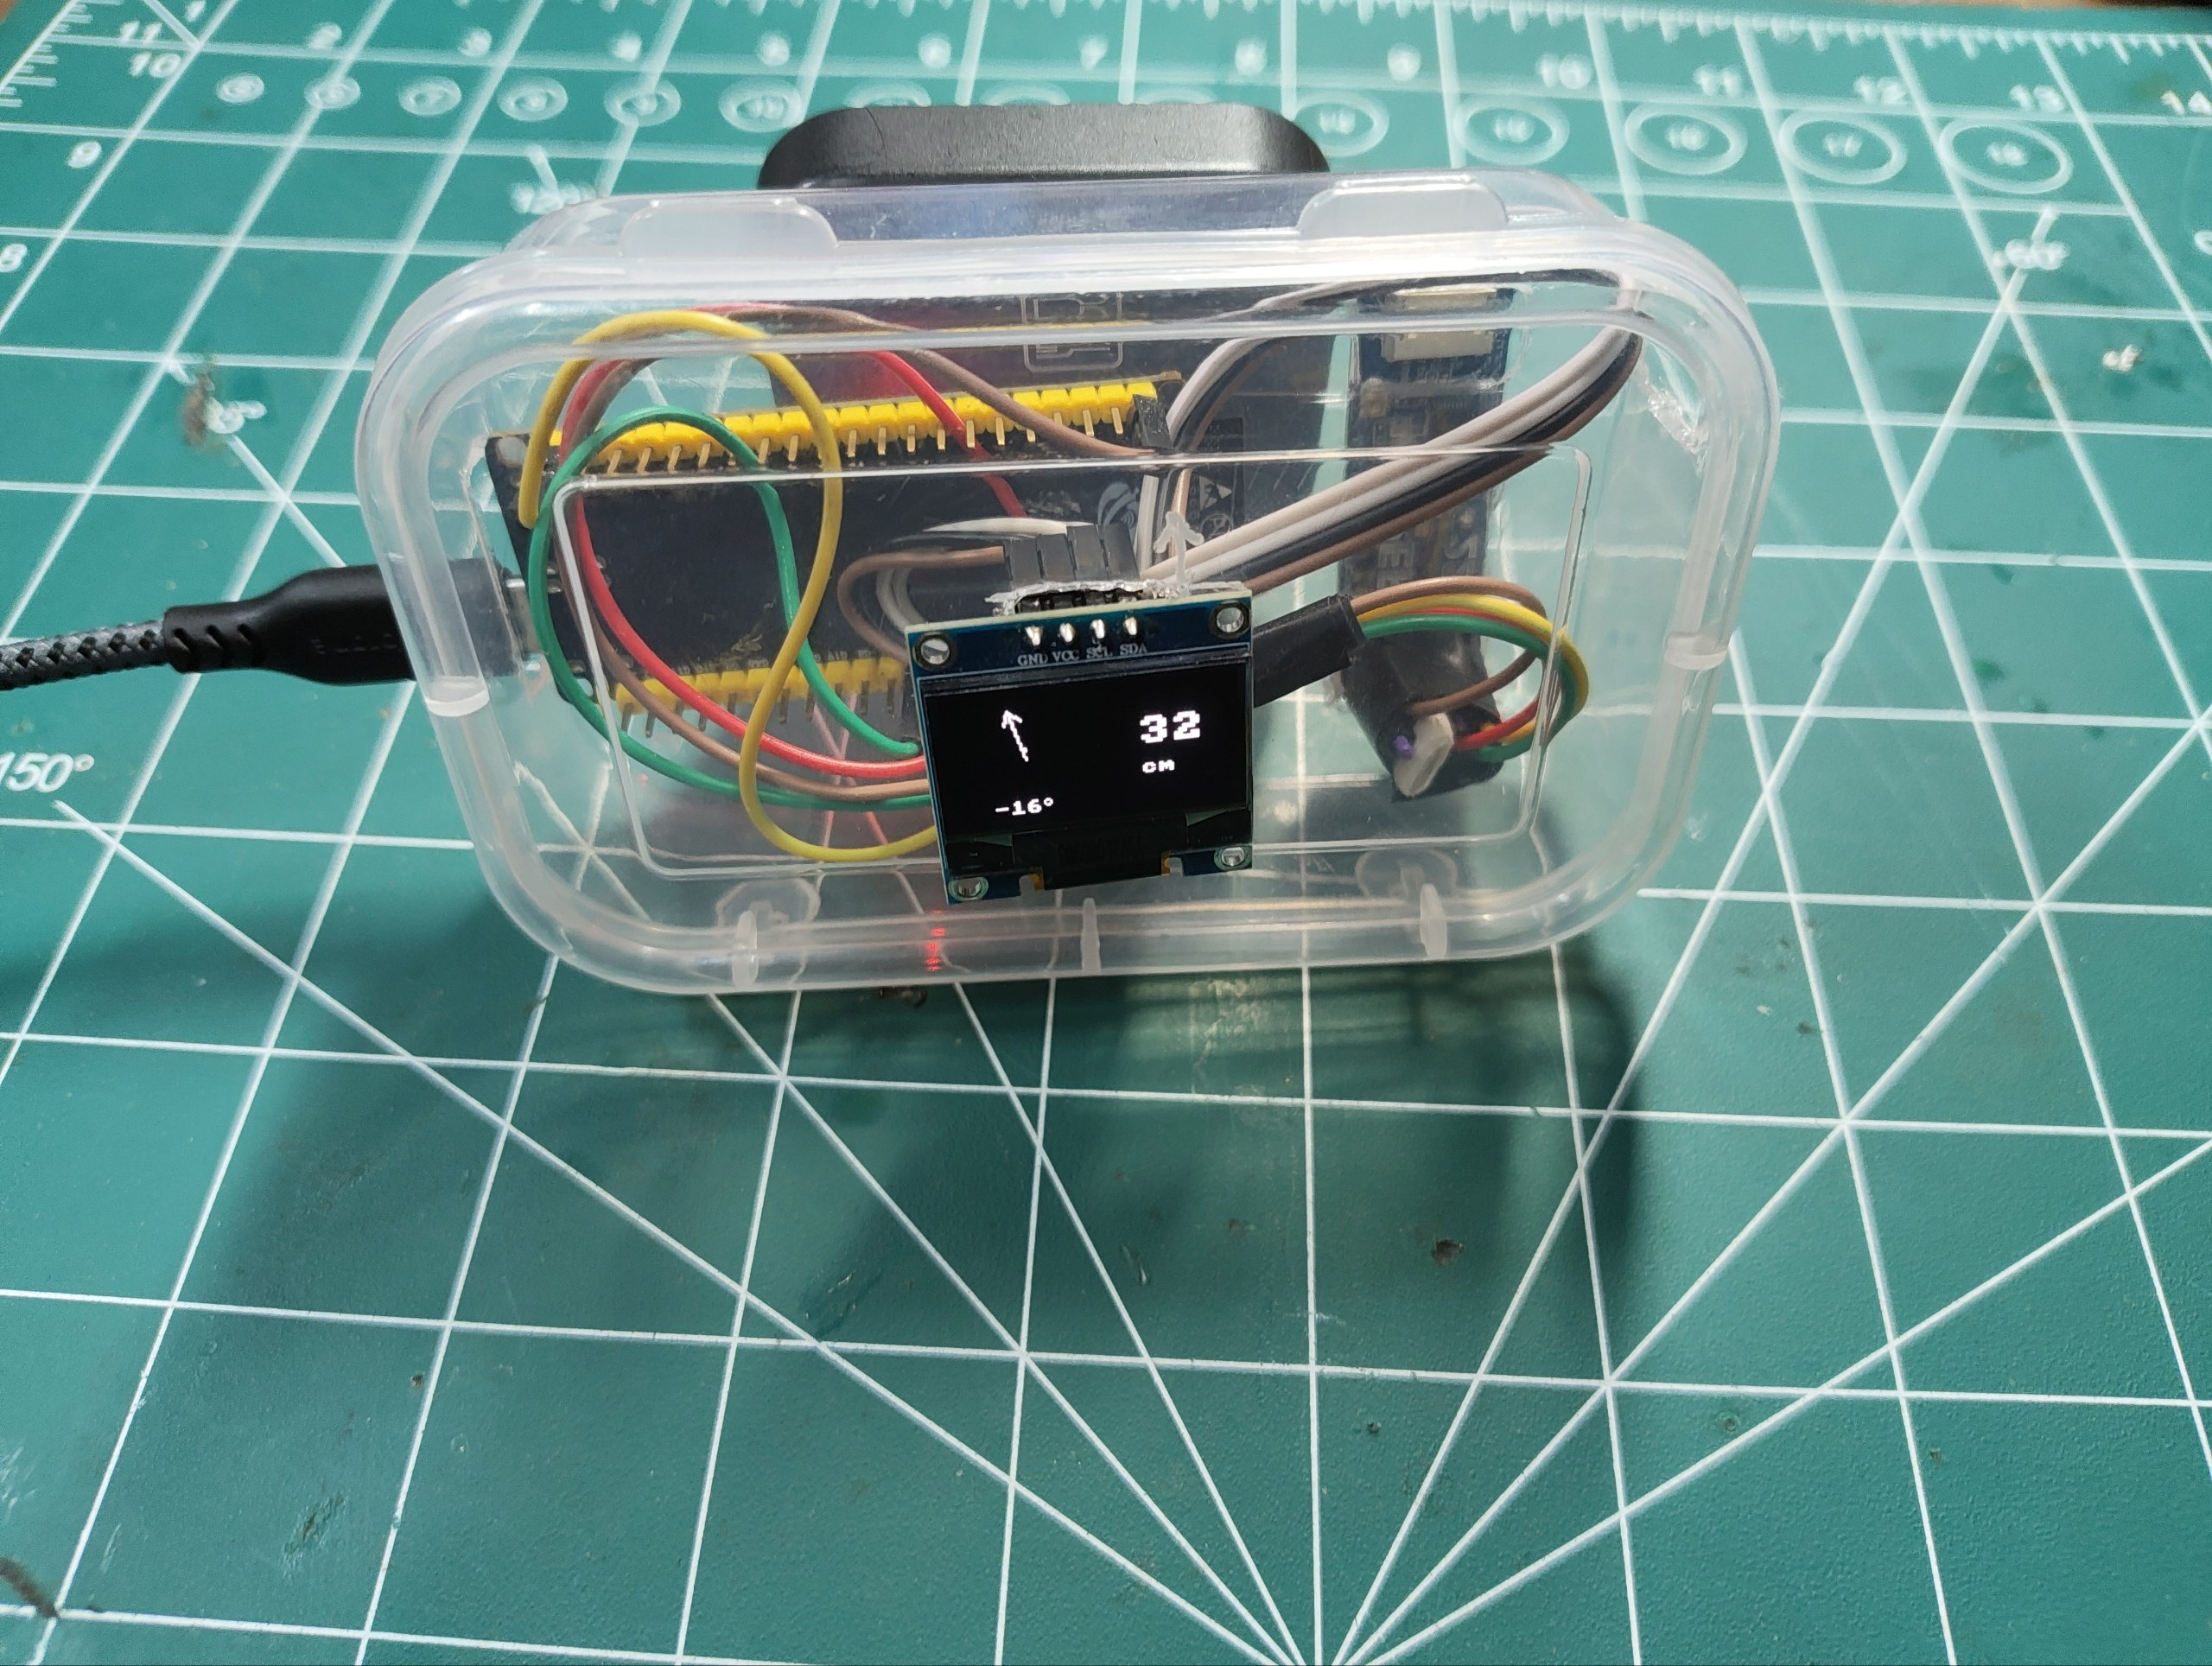
\includegraphics[width=0.75\textwidth]{Figures/SensorUnit.png}
\caption{Assembled sensor unit showing the ESP32-S3 microprocessor, HLK-LD2450 radar module, and active tag with trihedral corner reflector.}
\label{fig:sensor_unit}
\end{figure}

The 24~GHz FMCW radar in the HLK-LD2450 module communicates with its host via UART at 256,000 baud. This allows it to send out structured, 30-byte long frames (asynchronously) that support a tracking rate of up to 24~Hz. In terms of how those frames are parsed by the firmware's parser, it performs a sliding window byte-shifting using native memory moves to build each frame as they come in. The parser checks each packet received to ensure that it has a correct header identifier and performs a bitwise parity check; if either criteria are violated, the transmission will be rejected as invalid. The compute core begins FTM and controls the real time scheduler.

The millimeter-wave radar extracts Cartesian coordinate values of detected objects, while the UART bus provides asynchronous, serial communications. For every frame received correctly, the parser takes raw 16-bit signed integer representations of Euclidean coordinates from bytes 4 through 7 and converts these values into their equivalent Polar representation:

\begin{equation}
r = \sqrt{x^2 + y^2}, \qquad \theta = \arctan2(x, y) \times \frac{180}{\pi}
\label{eq:polar}
\end{equation}

Boundary filtering based upon hard coded limits eliminates readings below 0.1 meters distance from origin and/or beyond $\pm$60 degrees absolute angle. A critical limitation to the overall performance of the radar-based vision processing application is SRAM capacity. The on-device TFLite model was designed to be completely contained within SRAM so that all matrix multiplication required for ongoing prediction can occur without the significant latency associated with accessing external flash.

\subsection{Active Tag and Corner Reflector}
\label{sec:activetag}

The Cooperative Target includes an active tag which operates in the 802.11mc FTM Responder role; it is tied to a separate network (and therefore isolated) for its operation. When the FTM process begins, the tag hardware acknowledges each frame of the 16 exchanges initiated by the FTM initiator. The initiator computes distance using the total round-trip time of these exchanges, subtracts the processing delay of both devices, and uses the speed of light as a constant ($c = 299{,}792{,}458$ m/s). To minimize positive multipath bias, the firmware identifies the shortest (valid) temporal path for the tag among the sixteen timestamps:

\begin{equation}
r_{\text{path}} = \min(RTT_{1\ldots16}) \times 10^{-12} \times \frac{c}{2}
\label{eq:ftm_range}
\end{equation}

A passive trihedral corner reflector has been added to the active tag. This increases the Radar Cross Section (RCS) of the tag. Incoming 24~GHz radio frequency energy at the tag is reflected back to the source from three sides due to the orthogonally disposed reflective surfaces, producing a concentrated high-signal return that dominates background clutter - with zero power or computational overhead on the battery-powered tag.

\section{Dual Core FreeRTOS System Architecture}
\label{sec:freertos}

Real-time operation of multiple modes of data collection/processing on a single processor introduces significant conflicts regarding how the different system tasks can be scheduled. In particular, burst sequences associated with FTM operations require sub-microsecond level timing accuracy. Additionally, during these bursts it may be necessary to disable lower priority interrupts to ensure proper timestamping does occur. The UART (radar) interface sends one byte of data to be read by the software every 39 microseconds. If an interrupt cannot be issued within five milliseconds (a normal delay in software), it will overflow the hardware UART buffer and render the system unable to send or receive further commands.

\begin{figure}[htbp]
\centering
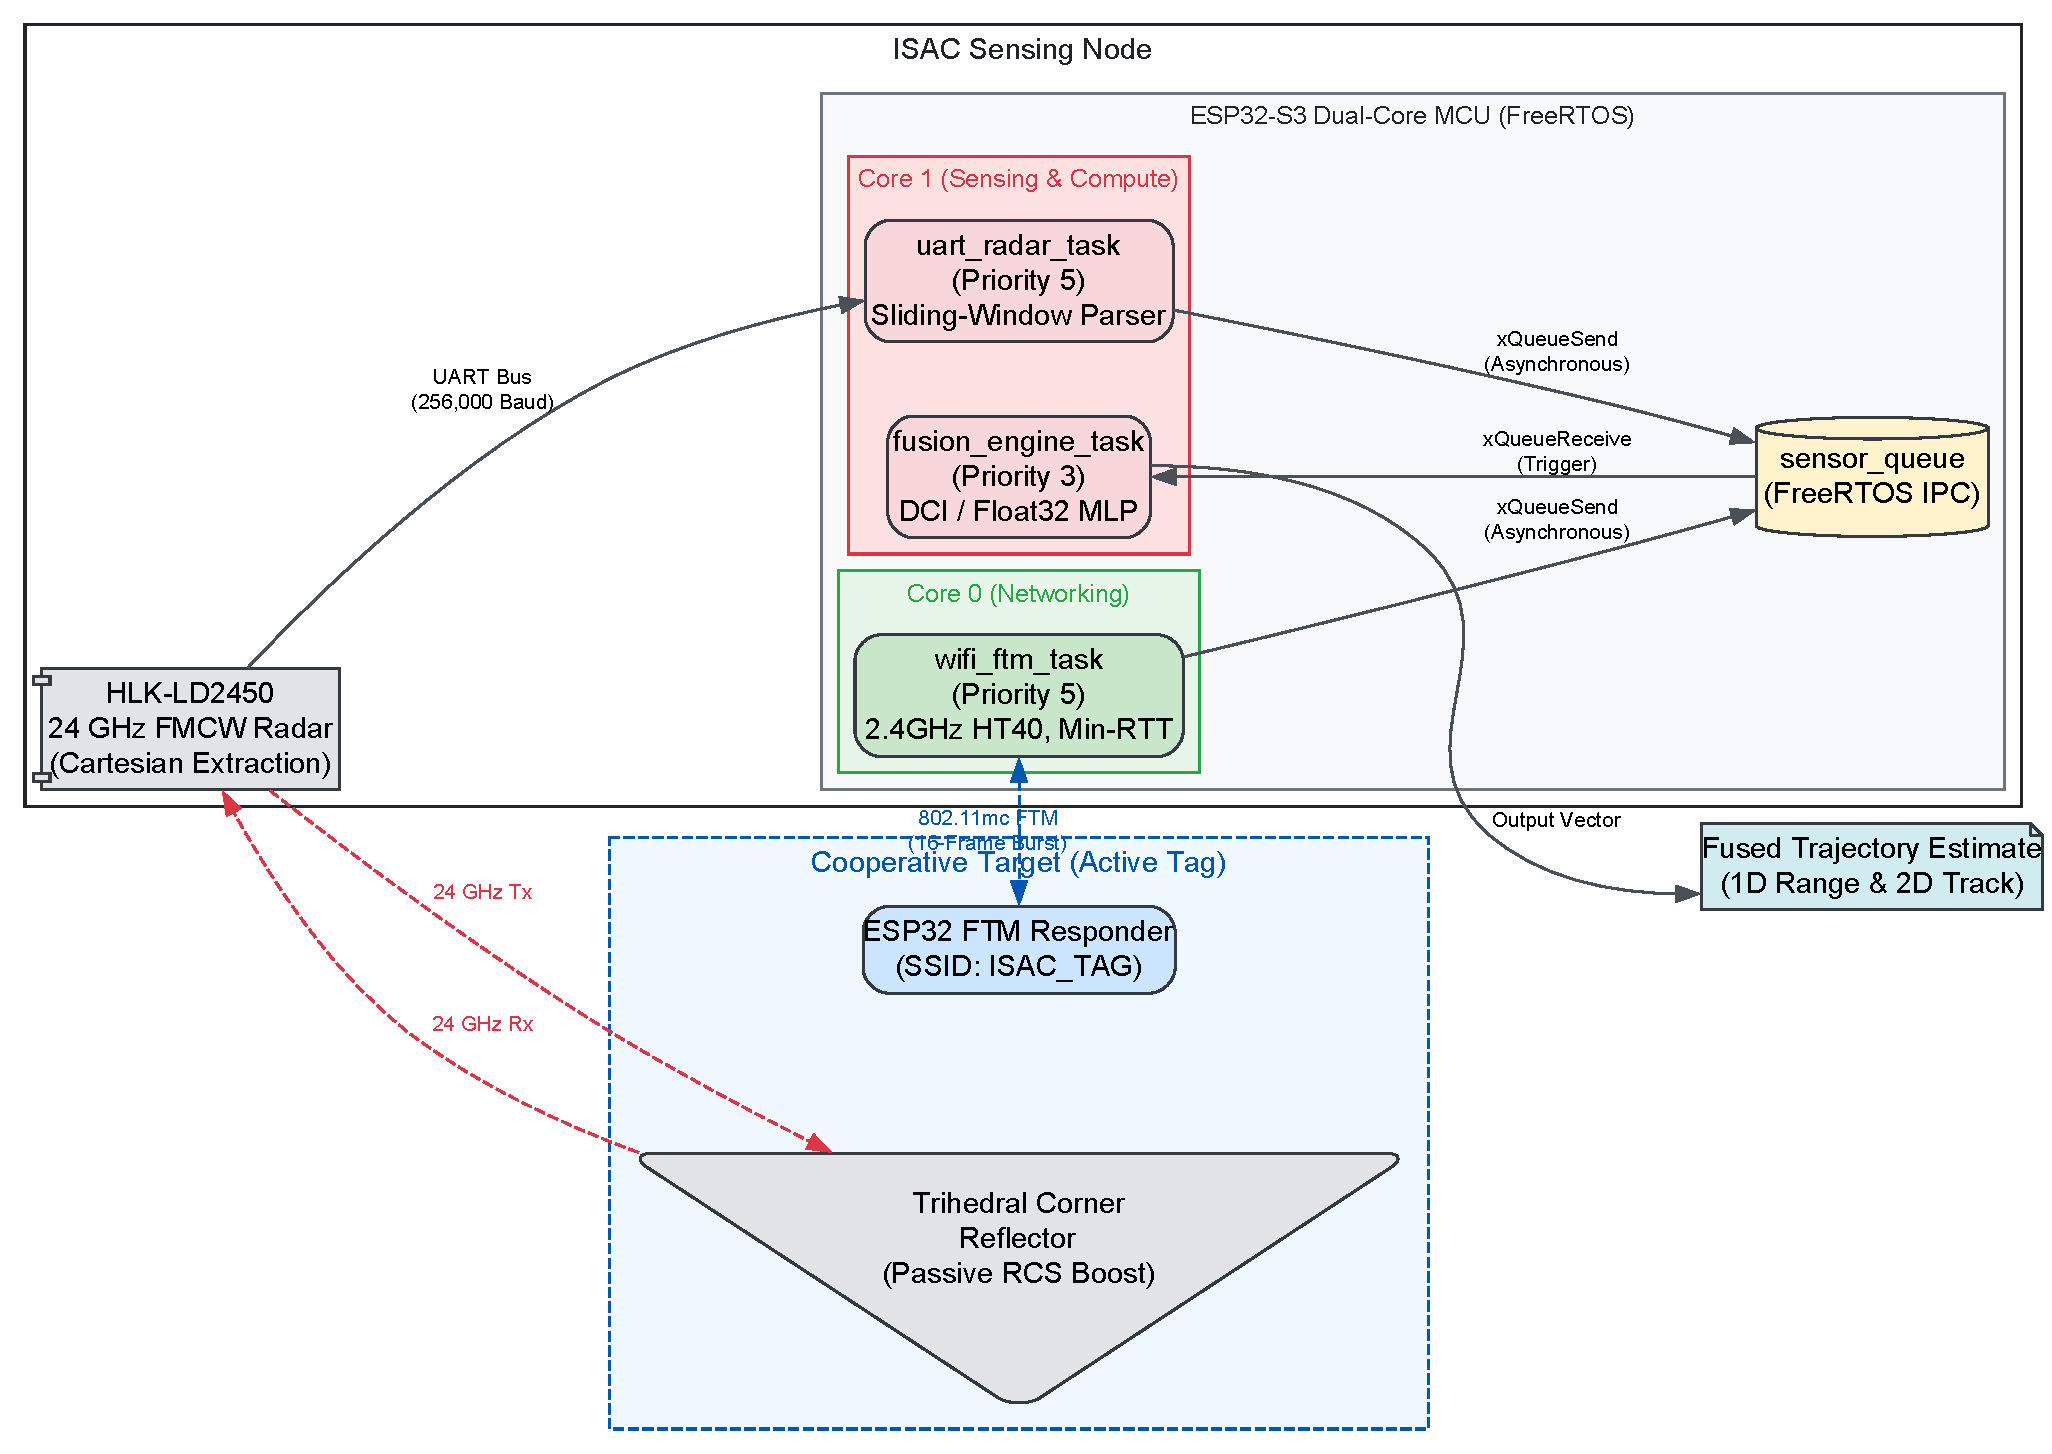
\includegraphics[width=0.85\textwidth]{Figures/SystemArchitectureFlowchart.pdf}
\caption{Dual-core FreeRTOS system architecture showing task isolation between Core~0 (Wi-Fi/FTM) and Core~1 (UART parsing and fusion engine).}
\label{fig:system_arch}
\end{figure}

Due to the fact that there can be no simultaneous execution of tasks on two cores of the processor, the solution to this problem was the permanent, absolute separation of the two cores. Processor Core~0 is permanently reserved for running the Wi-Fi task (Priority~5), and performs all FTM burst initiation functions, enforces channel integrity, extracts timestamps, etc. Processor Core~1 is used to run both the UART Radar Task (Priority~5), for managing buffers and parsing each frame into windows, and Fusion Engine Task (Priority~3), for performing tracking logic and inference.

All communication is performed by Core~0, which is also responsible for triggering sixteen-frame FTM bursts every 500~ms on the HT40 bandwidth to maximize timing resolution. Connection Management is restricted to this area of Core~0 so that Unpredictable Network Latency does not interfere with the Compute Pipeline. Core~1 ensures that UART Byte Shifting occurs prior to the Fusion Engine consuming this information, and the Fusion Engine performs Covariance Logic without being interrupted by Buffer Consumption. An RTOS Queue is used to bridge the Asynchronous Core Boundary. When a Producer Posts to the Queue it Posts with Zero Block Time - When the Queue Saturates Instead of Blocking Frames Are Dropped Rather Than Stalling the Parser. The Consumer of the Fusion Yields its CPU Allocation While Idle and Wakes Instantly Upon Arrival of New Data.
